\chapter{Clustering analysis} \label{s:clustering_analysis}

\vspace{3mm}
% \noindent\rule{17cm}{0.2pt}
\fbox {
    \parbox{\linewidth}{
      \begin{itemize}
        \item Cluster analysis with K-means  and PCA of the TCGA's MIBC cohort
        \item Three Basal splits based on the immune response
        \item Evidence for supporting the the Neuronal-like group
      \end{itemize}
    }
}
\vspace{3mm}

% Summary
% \subsection{Overview}

This section covers the work presented at the International Bladder Cancer Network (IBCN) in 2022 and is a major component of a research paper that will be submitted for peer review at the end of the PhD project. It describes the first attempt in the project to stratify the \acrfull{mibc} cohort from TCGA using only the gene expression (TPMs) obtained from RNAseq.

The proposed pipeline utilises standard clustering techniques, including K-means for clustering, Principal Component Analysis (PCA) for dimension reduction, and various clustering metrics. Despite relying on standard methods, novel subtypes within the major MIBC basal group were identified, potentially aiding biologists in better understanding the immune responses of basal tumours. This indirectly highlights the opportunity to identify new MIBC subtypes, demonstrating that even straightforward methods can yield significant results.



The chapter is structured into two main parts: the methods are detailed in \cref{s:cs:methods}, which includes justifications for selecting K-means as the clustering model, the number of groups, and the application of PCA prior to clustering. The configurations of the resulting pipeline are displayed in \cref{fig:cs:clustering_pipeline}. Kaplan-Meier survival analysis has shown that the derived MIBC subgroups exhibit significantly different survival prognoses, with the Neuronal and Basal groups with low Interferon-$\lambda$ demonstrating the poorest survival outcomes.

The final part of the chapter analyses and validates the groups derived and attributes biological functions using a series of tools: tumour purity scores from \citet{Yoshihara2013-wq}, Interferon-$\gamma$ response \citet{Baker2022-bj}, and other classifications from TCGA, Lund, and consensus \citet{Robertson2017-mg,Marzouka2018-ge,Kamoun2020-tj}. Both Differential Expression Analysis (DEA) and Gene Set Enrichment Analysis (GSEA) are employed to further validate the biological functions associated with the MIBC subgroups.

The in-depth code implementation of the cluster analysis (i.e., methods) run in this chapter can be found in the \textit{ReClassification\_42} Jupyter Notebook and the \textit{modelling.py} script file. All the plots and the code to determine the biological function of the derived MIBC subgroups are located in the \textit{Discussion\_42\_v2} notebook. All files are available at the \href{https://github.com/vladUng/Phd_thesis_exp}{GitHub repository} that accompanies the PhD project.


% Methods

% Experiments
\import{Sections/ClusteringAnalysis/}{experiments.tex}

% Interpretation
\import{Sections/ClusteringAnalysis/}{results.tex}

% Discussion
\section{Discussion}

% Basal groups
The main finding in this section is the identification of three Basal groups with differing immune responses. This discovery was facilitated by initially employing a standard clustering approach and subsequently comparing the results with existing MIBC classifications \citet{Baker2022-bj,Marzouka2018-ge}. Group-specific marker genes were identified using a suite of tools: DEA, pi-plots, GSEA, and other metadata available on TCGA.

% High and Medium IFNG
Both the High and Medium IFNG groups exhibit an \acrshort{ifn} response, highlighted by the expression of the \acrshort{ifn} signature from \citet{Baker2022-bj}. The two differ in that the High IFNG samples display a distinct immunoglobulin response, aligning them more closely with samples classified as Luminal Infiltrated. In contrast, the Low and Medium IFNG groups show stronger expression of basal/squamous subtypes compared to the third Basal group. Beyond the immune response differences, the DEA between Low/Med IFNG reveals few genes that are significantly expressed in the Low IFNG group. Some of these genes, highlighted in the analysis performed in \cref{s:cs:basal_interp}, may require further biological investigation, given the poor survival prognosis associated with Low IFNG.

% Urgency to study it
The fact that Low IFNG does not include Neuronal samples, according to our clustering and previous work, and that it has a survival prognosis as poor as that of the Neuronal group, underscores the novelty of this group and the urgency to study it.

% Neuronal group to study
In the TCGA classification, \citet{Robertson2017-mg} identified a Neuronal-like group comprising 20 samples, but our study found a larger group with 32 samples. The Kaplan-Meier survival analysis and the DEA/GSEA performed in \cref{s:cs:ne_interp} confirm the Neuronal-like nature of these subtypes. Compared to previous classifications, additional genes not included in the NE-like signature indicate tumour aggressiveness.

% Mention the LumP and LumInf 
The other two groups identified in this chapter, Luminal Papillary and Luminal Infiltrated, both display the differentiation markers (e.g., UPK, KRT) associated with these subtypes. The latter is distinguished from the former by exhibiting an immune response. The GSEA for the LumP group did not reveal any notable pathways, whereas for the LumInf group, it reinforced the characteristic immune response.


% Say that the output is in the figure
The results of this chapter are summarised in \cref{fig:cs:overview_K_means_6}, which displays the Kaplan-Meier survival analysis of the six groups at the top, and the Sankey diagram comparing our findings with the TCGA and Lund classifiers \citet{Robertson2017-mg,Marzouka2018-ge}. \cref{fig:cs:overview_survival} clearly shows that the Low IFNG and Neuronal-like groups have the poorest survival outcomes, while the LumP group exhibits the most favourable survival rates.


\begin{figure}[!htb]
    \centering
    \begin{subfigure}[!t]{1.0\textwidth}
        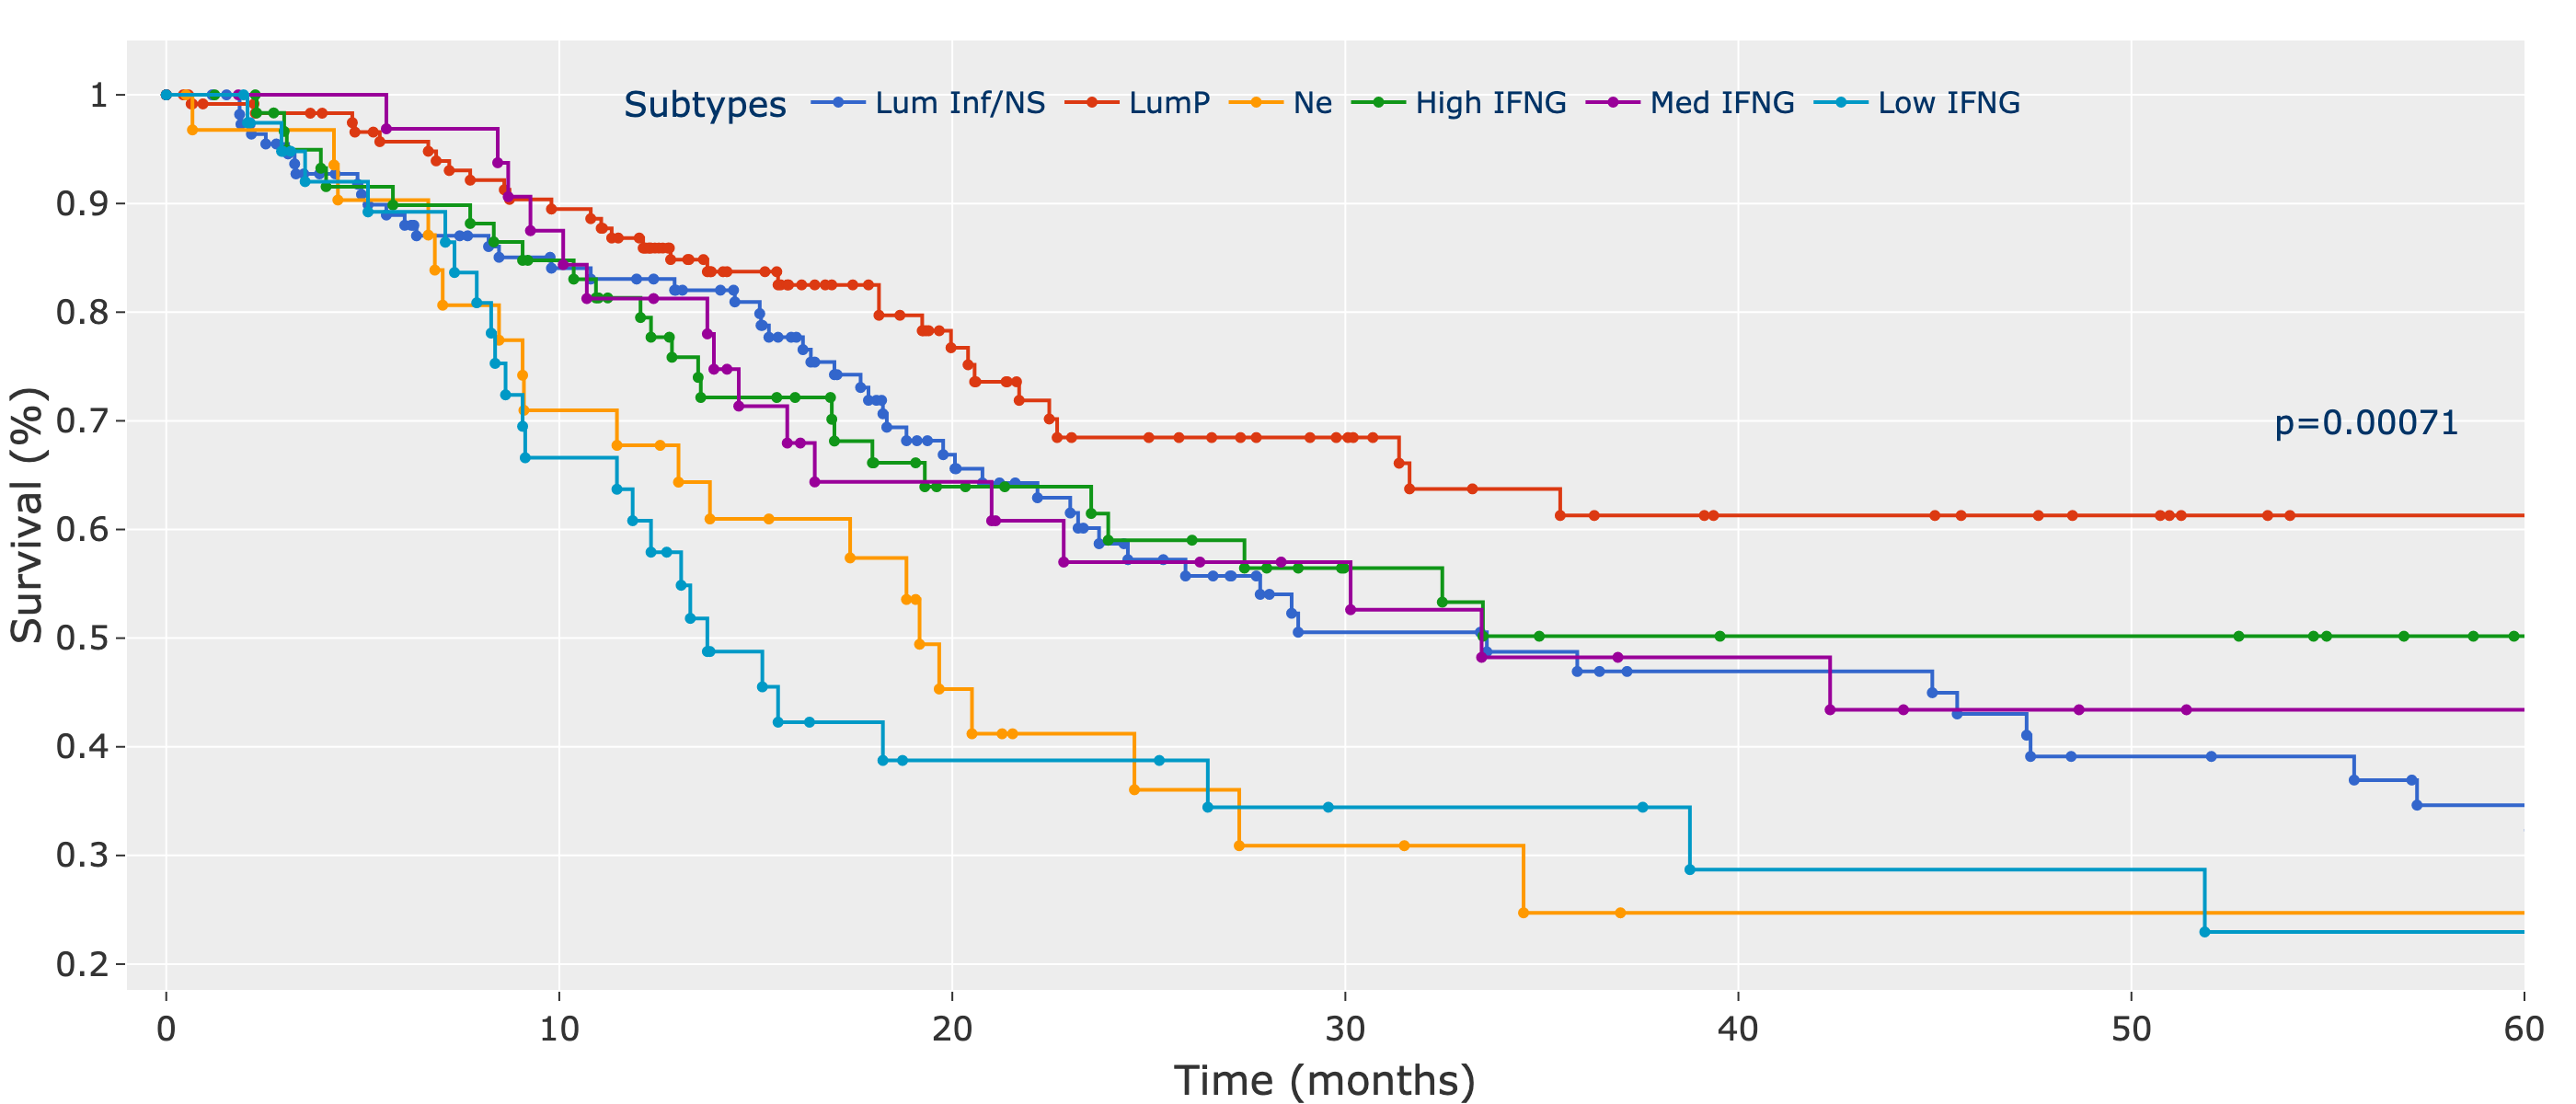
\includegraphics[width=\textwidth,keepaspectratio]{Sections/ClusteringAnalysis/Resources/discussion/survival_K_6.png}    
        \caption{Survival Kaplan-Meier}
        \label{fig:cs:overview_survival}
    \end{subfigure}
    \centering
    \begin{subfigure}[!t]{1.0\textwidth}
        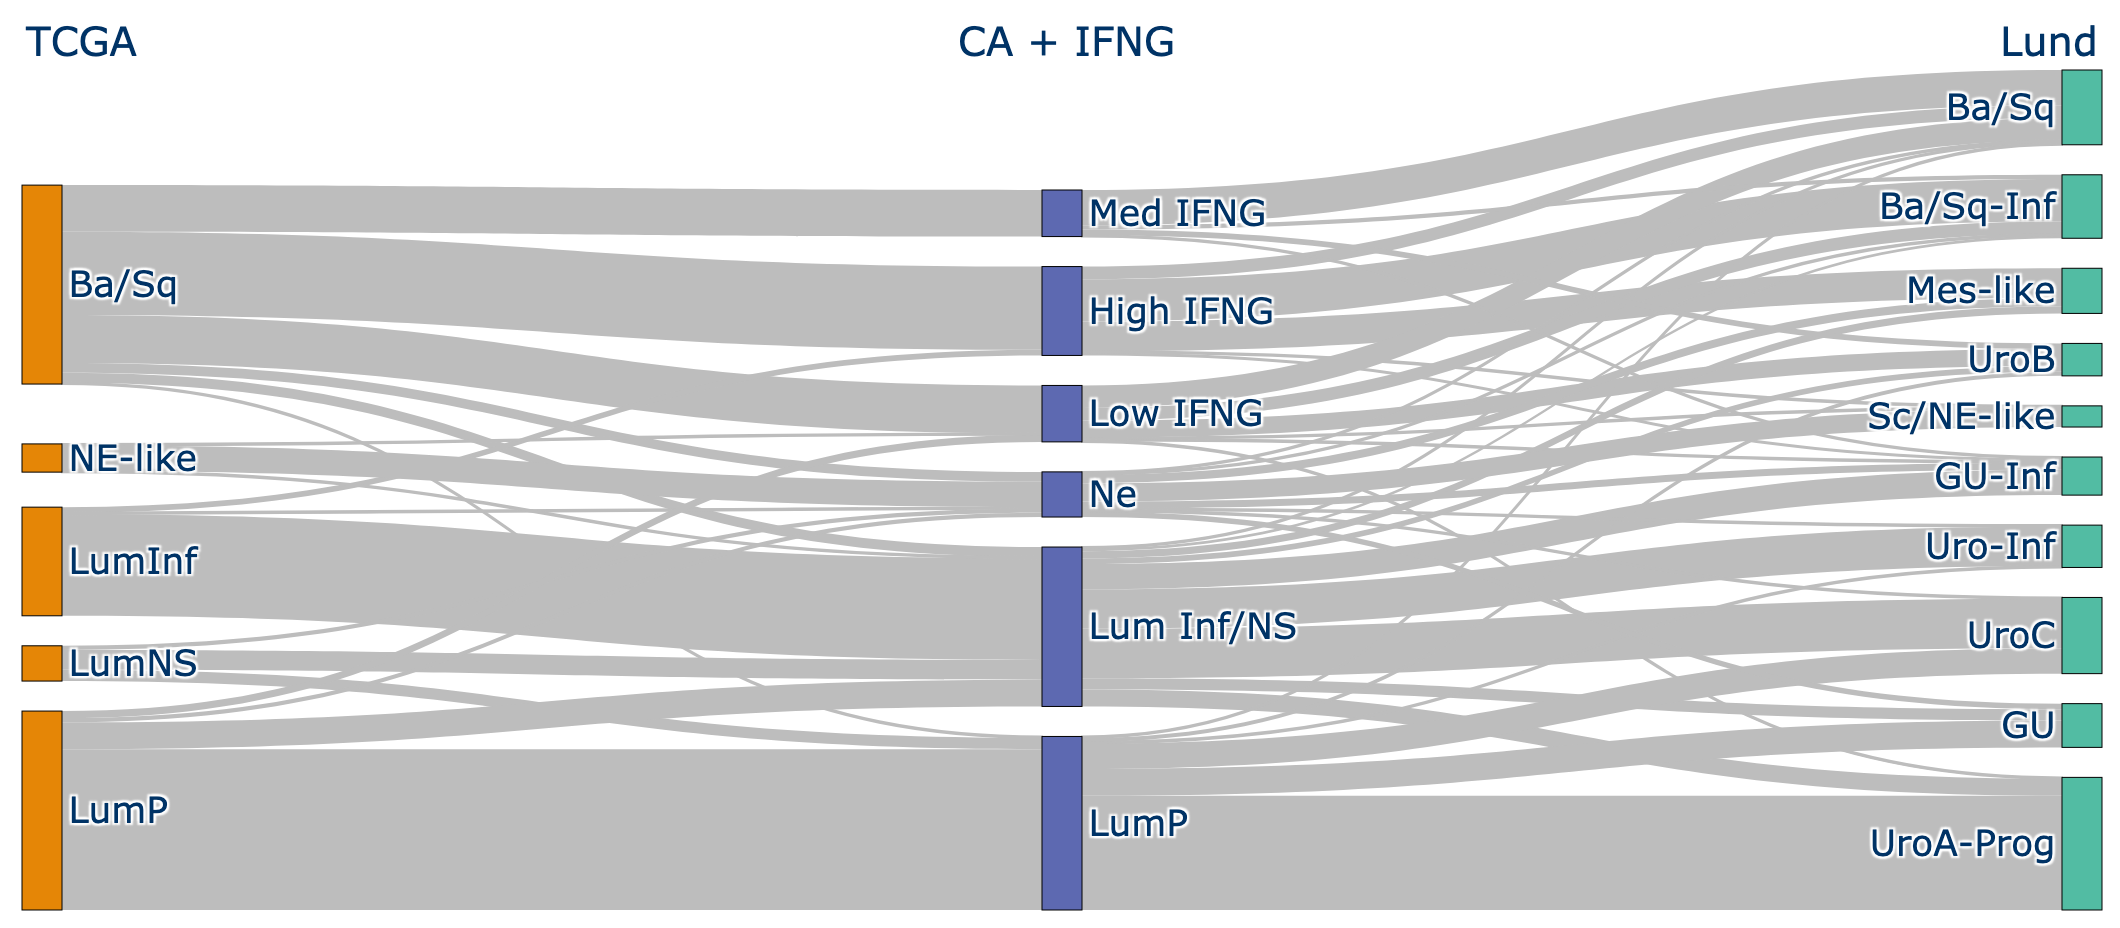
\includegraphics[width=\textwidth,keepaspectratio]{Sections/ClusteringAnalysis/Resources/discussion/KMeans_6_comp.png}
        \caption{Sankey plot}
        \label{fig:cs:overview_comp}
    \end{subfigure} 
    \centering
    \caption{Overview of the MIBC subtypes derived from using K-means K=5 and the \acrshort{ifn} Basal stratification form \citet{Baker2022-bj}. The first plot shows the Kaplan-Meier survival analysis of the 6 subgroups find, Ne and Low IFNG having the poorest prognosis. The Sankey at the bottom shows how the subtypes found are compared with the TCGA \citet{Robertson2017-mg} and Lund \citet{Marzouka2018-ge} classifiers.} 
    \label{fig:cs:overview_K_means_6}
\end{figure}


% Talk about gene filtering
This chapter employed an aggressive gene filtering approach by retaining genes expressed in at least 90\% of the samples. In contrast, the 'standard' method in the field involves removing genes from analysis that are expressed in less than 10\% of samples, making it more permissive. The aggressive filtering approach is an indirect finding of this chapter, as it enabled the clustering analysis to establish novel Basal groups based on their immune response.

% Talk about the implications of gene filtering
Applying a permissive gene filtering retains genes that are unexpressed in more than 10\% of the samples yet expressed in the remainder; these instances are characterised by high variance. Conversely, the aggressive gene filtering adopted here retains genes that are highly expressed across the samples, thus preserving a 'core' subset of genes across the MIBC subtypes. Consequently, the pre-processed data used for clustering analysis incorporated these 'core' genes, which contained immune response signals for the various Basal groups. This approach significantly impacts gene expression analysis as it underscores how different methods of gene filtering can lead to the discovery of new disease subtypes. Furthermore, it builds on previous work by \citet{Marzouka2018-ge,Baker2022-bj}, which differentiated the Basal group based on immune/infiltration responses using immunohistochemical (IHC) and \textit{in-vitro} experiments, respectively.

There are two main takeaways for the MIBC analysis, a change in gene filtering can have a large impact on the subgroups found and can yield novel subgroups. By using additional knowledge in some previous work \citet{Marzouka2018-ge,Baker2022-bj} new MIBC subtypes can be find. This attests that integrating additional data types may yield to a more complete molecular representation of the bladder cancer.


% Mention the methods that it will be useful for the following work
Apart from the novel Low IFNG group and the biological findings, this chapter represents the first attempt in the project to stratify the MIBC. The methods and visualisations tools are used throughout the project to perform cluster analysis and to interpret the new MIBC subgroups introduced in the following chapters.

